\documentclass[11pt]{article}
%Gummi|061|=)
\usepackage[table]{xcolor} 
\usepackage{vmargin}
\usepackage[T1]{fontenc} %encoding del font
\usepackage[utf8]{inputenc} %encoding dell'input
\usepackage[italian]{babel} %lingua per la formattazione
\usepackage{mparhack}
\usepackage{pgfplotstable}
\usepackage{float}
%pacchetti per la formattazione
\usepackage{calc} %fantasmi

\usepackage{graphicx} %inserire immagini (grafici vettoriali.pdf)
%pacchetti -->\SCfigure \SCtable
\usepackage{booktabs} %pacchetto per per le tabelle
\usepackage{amsmath, amssymb} %pacchetti per usare comandi matematici
\usepackage{pgf,tikz}
\usepackage{caption}
\usepackage{siunitx}
\usepackage{setspace}
\usepackage{subfig}
\usepackage{array}
\usepackage{multirow}

\title{\textbf{Equazione di stato dei Gas}\\ Autori}
\author{ xxxxxxxxxxxxx\and
		xxxxxxxxxxxxx\and
		xxxxxxxxxxxxx}
\date{\today}
\setmarginsrb{30mm}{10mm}{20mm}{10mm}%
             {0mm}{10mm}{0mm}{10mm}

\newcommand{\HRule}{\rule{\linewidth}{0.5mm}}
             
\begin{document}
\begin{titlepage}
\begin{center}

% Upper part of the page. The '~' is needed because \\
% only works if a paragraph has started.

\includegraphics[width=0.20\textwidth]{./Logo1}~\\[1cm]

\textsc{\LARGE University of Trento}\\[1.5cm]

\textsc{\Large Appunti dalle lezioni di Fisica II}\\[0.5cm]
\vspace{30pt}
% Title
\HRule \\[0.4cm]
\vspace{15pt}
{ \huge \bfseries Fisica II}\\[0.4cm]
\vspace{15pt}
\HRule \\[1.5cm]
\vspace{30pt}
% Author and supervisor
~~~~~~~~~~~~~~~~~~~~~\begin{minipage}{0.4\textwidth}
\large
\emph{\large\textbf{Autori}}\\ \\ 
A.\textsc{V.}
\end{minipage}

\vfill

% Bottom of the page
{\large \today}

\end{center}
\end{titlepage}\newpage
\tableofcontents
\newpage
\vspace{40pt}
\rowcolors{1}{gray!25}{white}
~\\
%\textbf{Introduzione}\\\\
\section{Introduzione}
Se strofinassimo un palloncino di plastica sul nostro maglione ci accorgeremmo che qualcosa nel palloncino è cambiato.\\Ad esempio se lo appoggiassimo ad un anonimo muro bianco dell'aula A105 del polo Ferrari di Povo ci accorgeremmo che esso si attacca al muro e ci resta pure, almeno per un po'.\\La fisica che sta alla base di questo fenomeno sottende ad una vastistissima gamma di applicazioni e strumenti: computer, ascenzori e via dicendo.\\Il palloncino era un esempio ma la stessa cosa accade se usiamo del vetro, l'unica differenza è che i due diversi materiali si ``caricano'' in modo diverso, ispirando la prima e più elemntare suddivisione tra la tipologia di ``elettrizzazione'' vetrosa (positiva) e resinosa (negativa).
Si osserva poi che oggetti caricati nello stesso modo si respingono mentre si attirano se caricati uno negativamente e l'altro positivamente.
\section{Proprietà dei materiali}
Ci sono oggetti che favoriscono lo scorrere di elettroni (di carica), al loro interno e altri che ne ostacolano il flusso.\\In generale ci si riferisce con il termine dielettrico ad un materiale \textbf{non conduttore} ma in realtà tutti gli oggetti hanno un grado di ``non-conducibilità''.\\Tale attributo induce la categorizzazione dei materiali: quelli propriamente non conduttori e quelli conduttori (e le classi di confine e quelle intermedie) che mostrano macroscopicamente proprietà peculiari. Da qui in poi si identificherà la parola conduttore con quella di \textbf{metallo} e la parola non conduttore con quella di \textbf{dielettrico}.
\subsection{Proprietà dei materiali dielettrici}
Un fenomeno che concerne i materiali dielettrici è quello di \textbf{polarizzazione}.\\Ripensiamo all'esempio del palloncino. Perchè rimaneva attaccato al muro? Forse il muro era già caricato negativamente per conto suo? Oppure è stato in qualche modo l'oggetto carico ad influenzare le cariche disposte su di esso?
E' avenuto il fenomeno di polarizzazione. Nel nostro caso il muro è un non conduttore, ciò significa che la carica su di esso non è libera di scorrere liberamente e gli atomi al suo interno sono disposti schematicamente come in figura.
\begin{center}
\begin{figure}[H]
			  \vspace{0pt}
              \hspace{-90pt}
              ~~~~~~~~~~~~~~~~~~~~~~~~~~~~~~~~~~~~~~~~~~~ 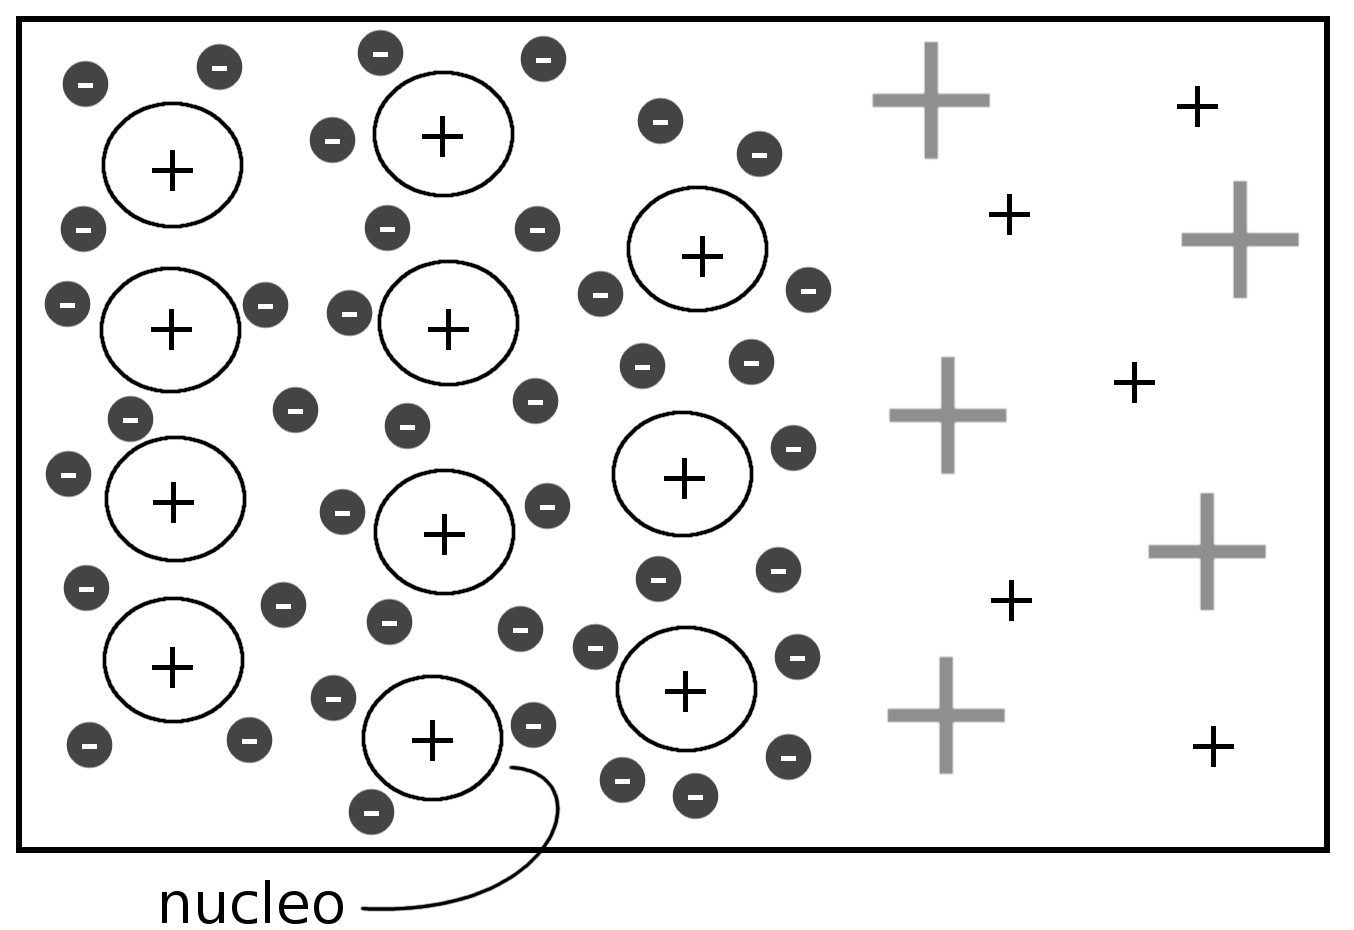
\includegraphics[scale=0.21]{dielettrico}
               \caption{Schematizzazione della distribuzione delle cariche nel materiale dielettrico}
               \end{figure} 
               \end{center}
               Gli atomi sono distribuiti in modo uniforme e altrettanto uniformemente sono distribuiti attorno ad essi le cariche negative (gli elettroni); così appare in generale il materiale non sottoposto ad alcuna forza elettromagnetica.
\\Se provassimo ad avvicinare un corpo carico, ad esempio positivamente osserveremmo che la nube elettronica, in principio disposta in modo simmetrico attorno al nucleo si deforma e si sposta verso. Il carattere di non conduttore del materiale impedisce che gli elettroni vaghino liberamente da un estremità all'altra dell'intero corpo confinando gli spostamenti nel raggio atomico come mostrato in figura.
\begin{center}
\begin{figure}[H]
			  \vspace{-10pt}
              \hspace{-90pt}
              ~~~~~~~~~~~~~~~~~~~~~~~~~~~~~~~~~~ 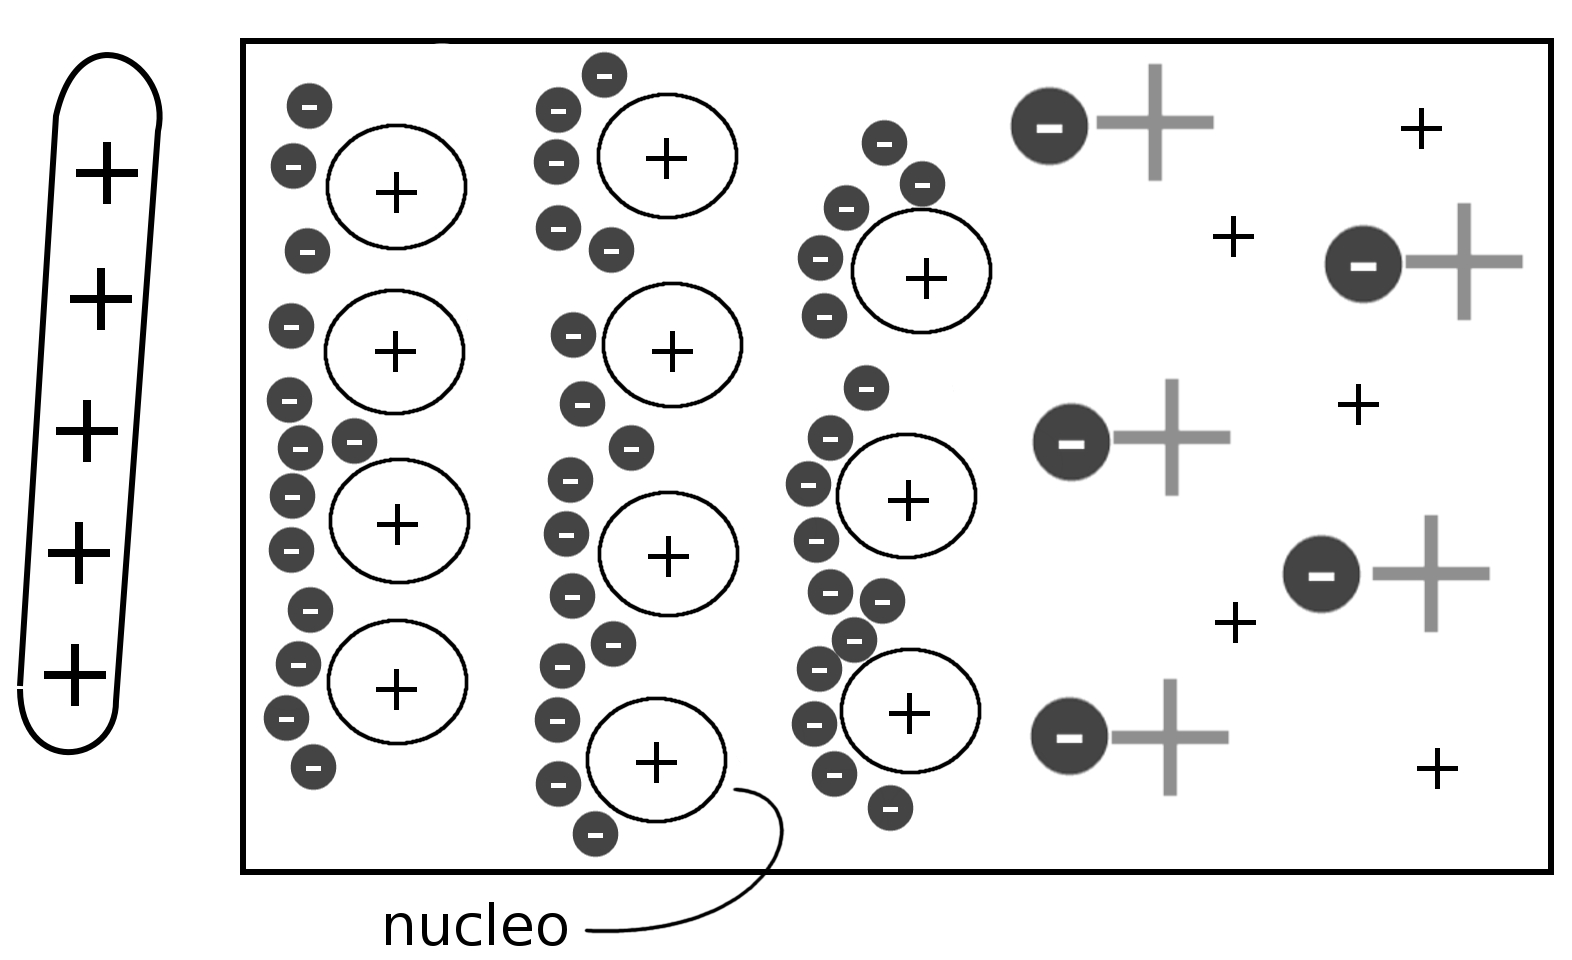
\includegraphics[scale=0.21]{dielettrico2}
               \caption{\small{Schematizzazione della distribuzione delle cariche nel materiale dielettrico in presenza di una distribuzione di carica esterna}}
               \end{figure} 
               \end{center}
               \vspace{-30pt}La figura illustra molto chiaramente il fenomeno in questione e fa luce sull'esempio ~del palloncino. Il palloncino viene caricato e posto in vicinanza del dielettrico, polarizzandolo; così facendo la superficie del muro risulta caricata negativamente (localmente) ed essendo il palloncino caricato positivamente i due materiali si attraggono.
               \subsection{Proprietà dei materiali conduttori}
               Al contrario dei materiali dielettrici i metalli non ostacolano il flusso di elettroni al loro interno (non confinandoli attorno ai nuclei). In questo modo, avvicinando un corpo carico al metallo, le cariche negative vengono attratte verso di esso.\\Questo processo è noto come \textbf{induzione elettrostatica} e risulta ben descritto dalla figura 3
\begin{center}
\begin{figure}[H]
			  \vspace{-10pt}
              \hspace{-90pt}
              ~~~~~~~~~~~~~~~~~~~~~~~~~~~~~~~~~~~~~~~~~~~~ 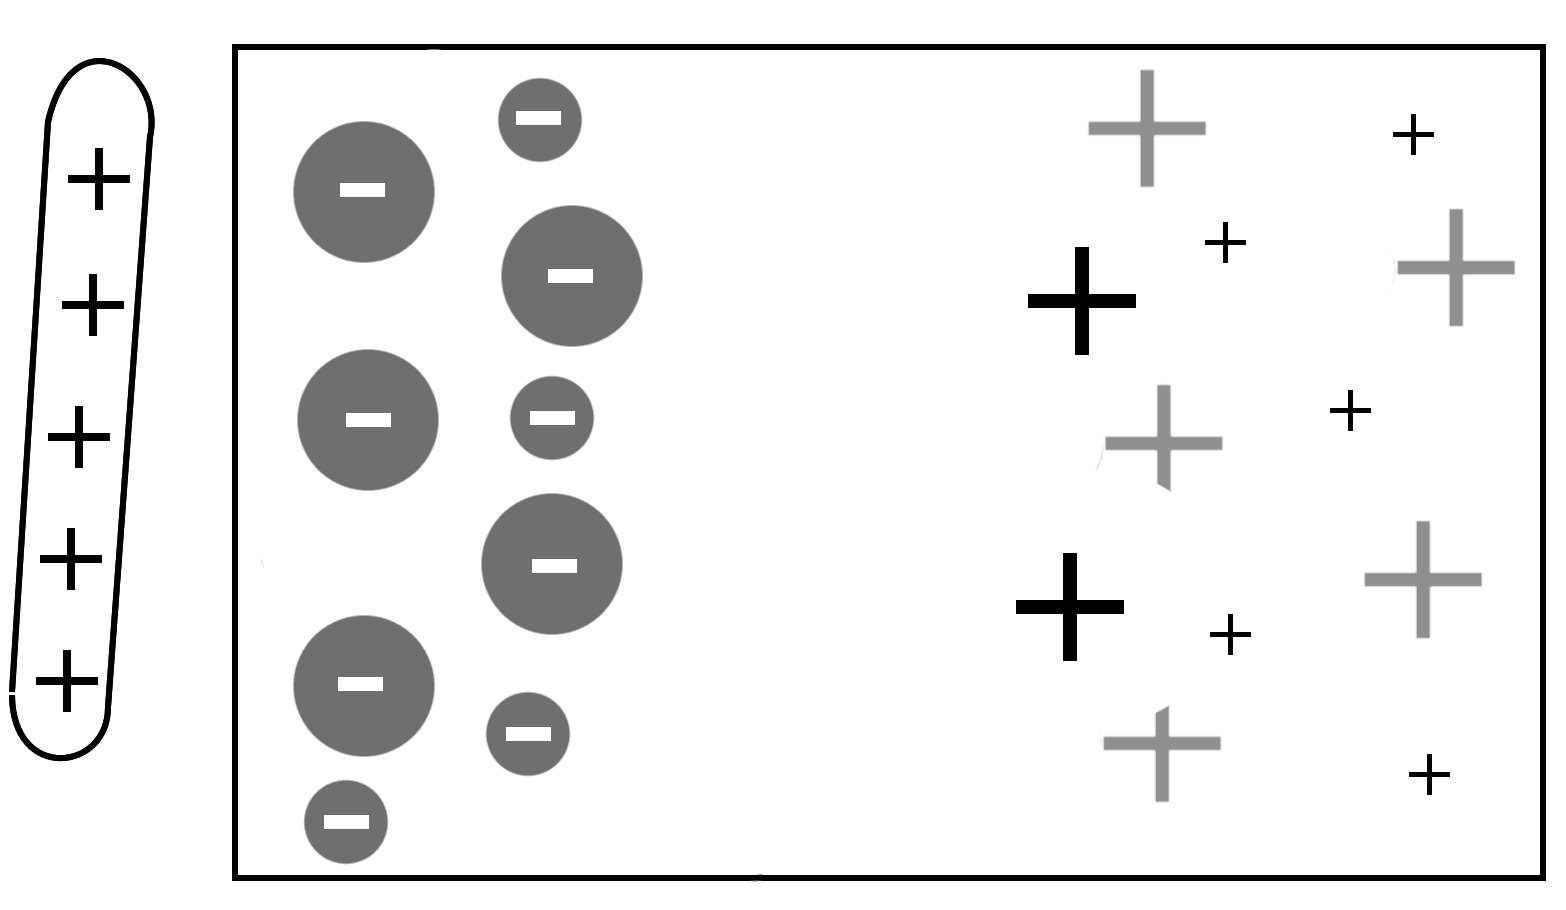
\includegraphics[scale=0.17]{dielettrico3}
               \caption{\small{Schematizzazione della distribuzione delle cariche nel materiale dielettrico in presenza di una distribuzione di carica esterna}}
               \end{figure} 
               \end{center}
               \section{La carica elettrica}
               Una volta osservato qualitativamente l'effetto che produce l'interazione fra caricche è utile trovare un modo per quantificarne l'entità. Un modo per poter stimare il valore della carica è l'utilizzo dell'elettroscopio.\\L'elettroscopio è uno strumento composto da una sfera metallica collegata tramite un conduttore ad un estremita costituita da due foglie sottili di conduttore (solitamente oro) sotto vetro. Caricare la testa dell'elettroscopio fa aumentare la carica totale dello strumento che si distribusice su tutto il metallo, in particolare sulle due sottili foglie conduttrici. Poichè entrambe le foglie sono caricate negativamente si respingono e si può stimare indirettamente la quantità di carica misurando l'angolo di deflessione delle lamine.
               \begin{center}
\begin{figure}[H]
			  \vspace{-10pt}
              \hspace{-90pt}
              ~~~~~~~~~~~~~~~~~~~~~~~~~~~~~~~~~ 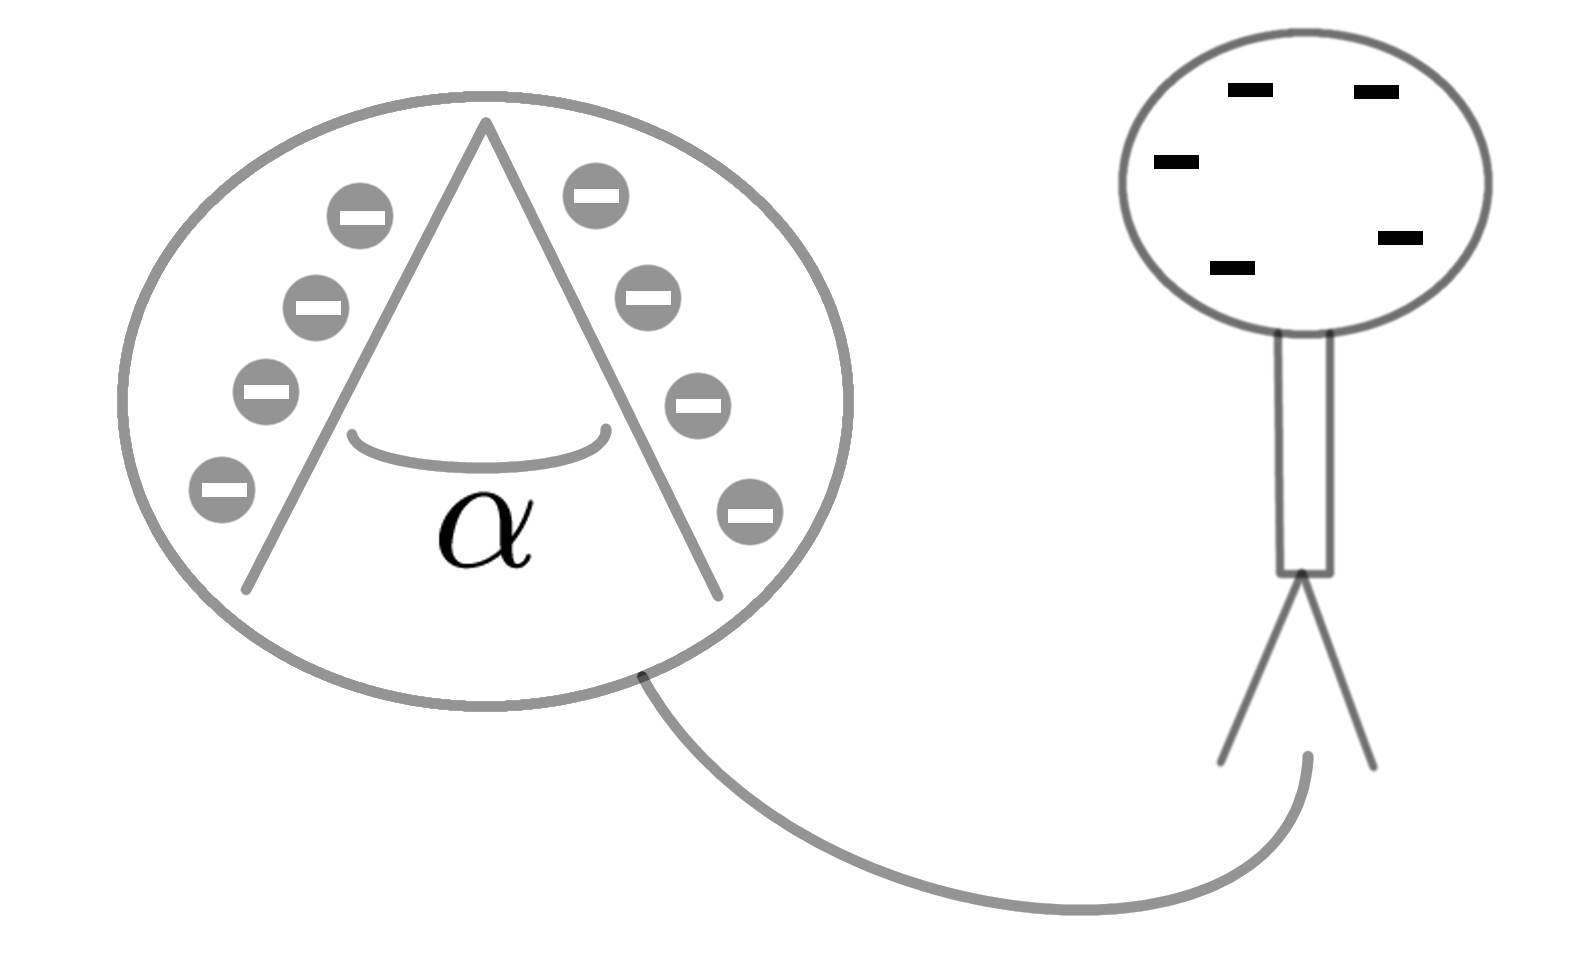
\includegraphics[scale=0.22]{elettroscopio}
               \caption{\small{Rappresentazione schematica di un elettroscopio e dell'angolo di flessione.}}
               \end{figure} 
               \end{center}
               Si può tracciare un grafico che metta in relazione l'angolo di deflessione con la quantità di carica. \\E' utile ricordare che la natura dell'elettroscopio è di un rilevatore ci carica, più che un misuratore poichè meno si presta alla misura quantitativa propria di un elettrometro.
                \begin{center}
\begin{figure}[H]
			  \vspace{-10pt}
              \hspace{-90pt}
              ~~~~~~~~~~~~~~~~~~~~~~~~~~~~~~ 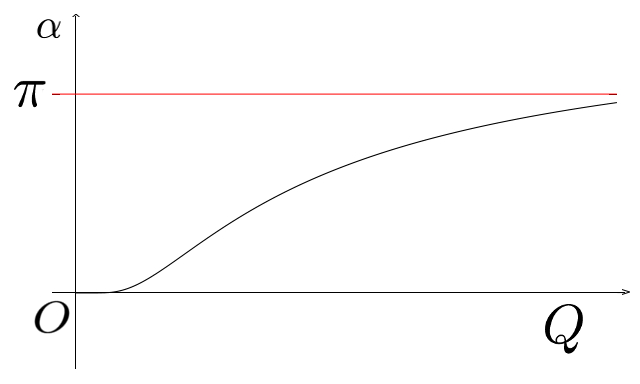
\includegraphics[scale=0.60]{flessione}
               \caption{\small{Grafico dell'andamento della flessione delle lamine in funzione della carica}}
               \end{figure} 
               \end{center}
               \subsection{La carica è quantizzata}
Esiste un unità fondamentale e indivisibile della carica, essa vale $1.6 \times 10^{-19}$ C e corrisponde alla carica dell'elettrone. 
$$Q=ne$$Tutti gli elettroni hanno quindi la stessa carica sicchè se volessimo calcolare il numero di elettroni necessari alla produzione di un Coulomb potremmo ricavarlo elementarmente come segue:
$$n=\frac{1~C}{1.6 \times 10^{-19}~C}=6 \times 10^{18}~elettroni$$
Per avere un idea più concreta torniamo al palloncino di prima; durante lo sfregamento del palloncino sul maglione viene trasferita una carica di circa $10^{-7}$ C che corrisponde grossomodo a $0.6 \times 10^{12}$ elettroni.
\section{Forza elettrica}
Un buon metodo per calcolare la forza elettrica è l'utilizzo di una bilancia stile Cavendish con la quale identificare una corrispondenza tra forza elettrica e momento torcente della bilancia.
\begin{center}
\begin{figure}[H]
			  \vspace{-10pt}
              \hspace{-90pt}
              ~~~~~~~~~~~~~~~~~~~~~~~~~~~~~~~~~ 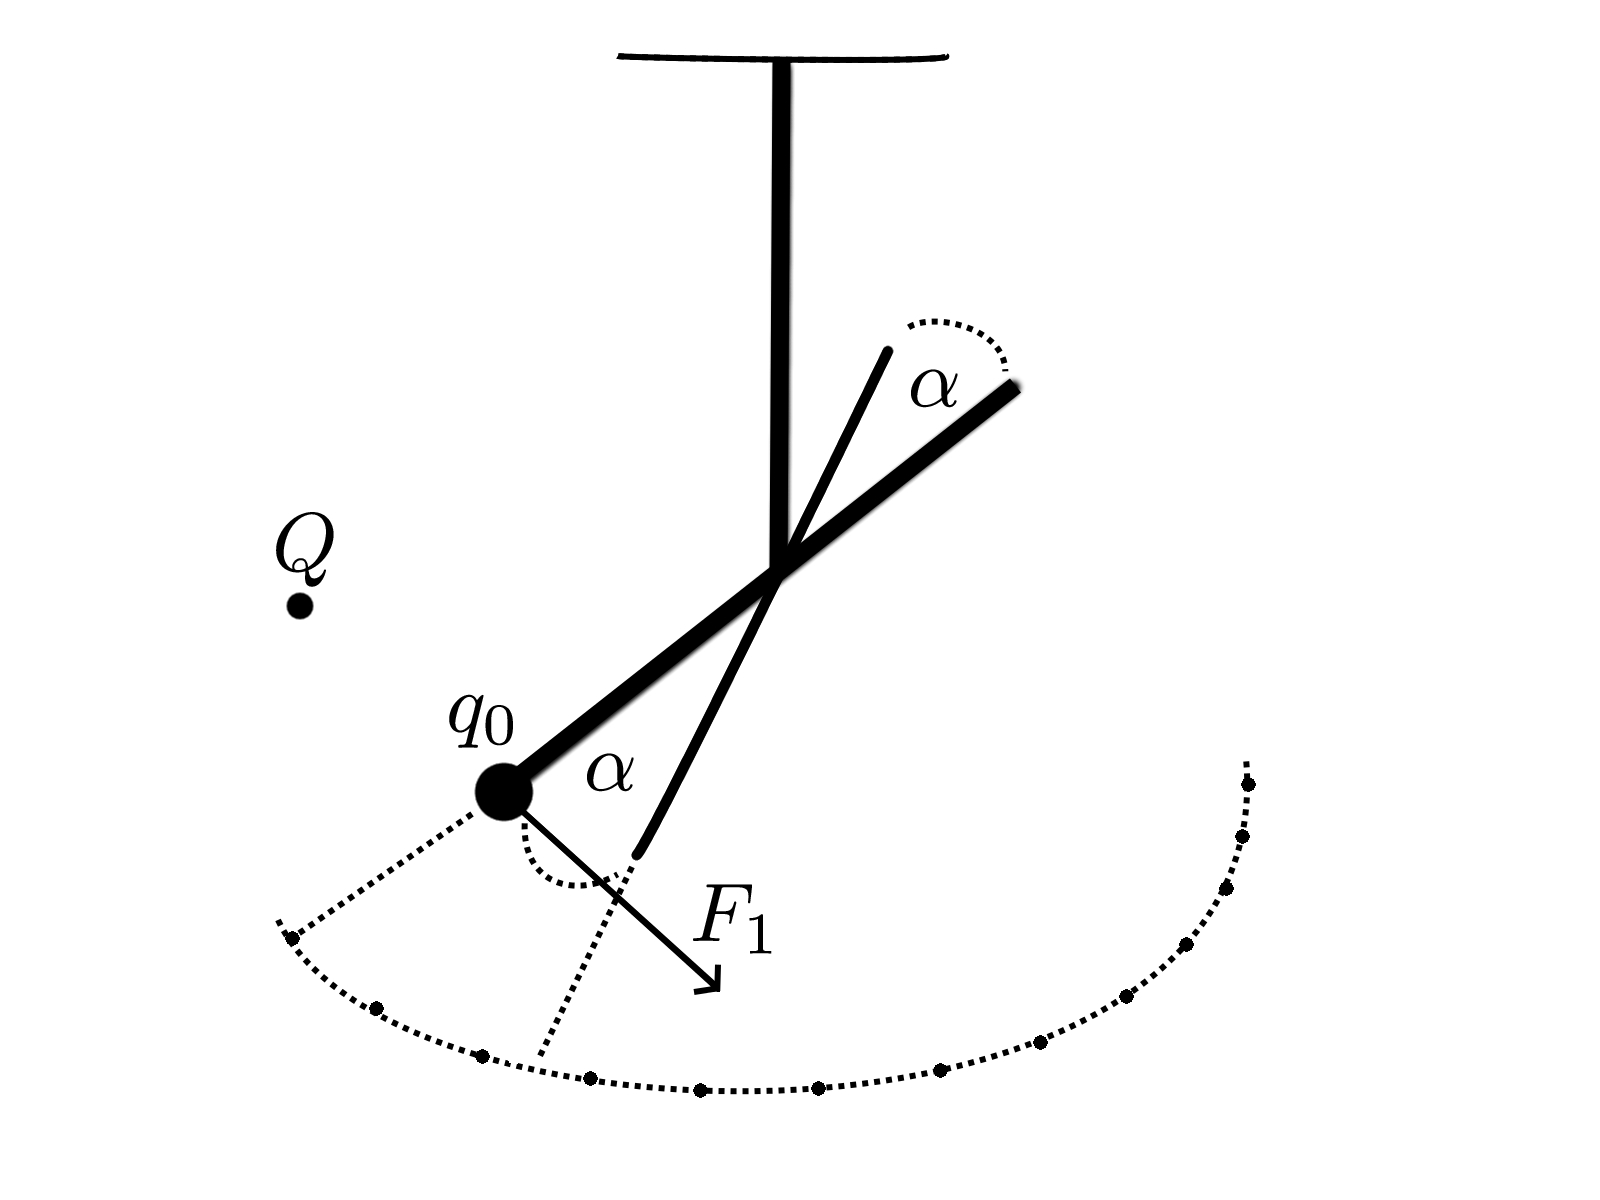
\includegraphics[scale=0.22]{cavendish}
               \caption{\small{Rappresentazione schematica di una bilancia alla cavendish per la misura di forza elettrica.}}
               \end{figure} 
               \end{center}
Dagli esperimenti si ricava la seguente relazione funzionale:
$$F_e=k_e\frac{qQ}{r^2}$$
dove $k_e=9\times10^9~~\frac{Nm^2}{C^2}$
\\è interessante osservare l'analogia con la forma del espressione per la forza gravitazionale:
$$F_g=G\frac{mM}{r^2}$$
E' interessante calcolare il valore del rapporto tra forza elettrostatica e gravitazionale tra due elettroni per avere un idea indicativa della preponderanza di una rispetto all'altra.
$$\frac{F_e}{F_g}=\frac{\frac{k_e(1.6\times10^{-19}(1.6\times10^{-19})}{r^2}}{\frac{}{r^2}}~~~da~controllare$$
\subsection{Formalizzazione vettoriale}
$$\overrightarrow{F}_q=k_e\frac{qQ}{|\overrightarrow{r}|^2}\hat{r}$$
Per la forza elettrostatica vale l'usale principio di sovrapposizione delle forze e si può definire, come per il campo gravitazionle, il campo elettrostatico.
E' facile arrivare alla conlusione che l'unico modo di esprimere un campo elettrico in modo univoco è dividere per la ``carica di prova'' $q_0$ in modo tale che si possa scrivere:
$$\overrightarrow{E}=\frac{\overrightarrow{F}}{q_0}$$
\section{Distribuzioni di cariche}
Abbiamo già visto l'espressione per la forza generata da una carica puntiforme. ora possiamo sciverla nella sua forma estesa e valutarne il grafico.
$$\overrightarrow{F_e}=\frac{1}{4\pi\epsilon_0}\frac{Qq_0}{r^2}\hat r$$
dove $\epsilon_0=9.95\times 10^{-12}$
\begin{center}
\begin{figure}[H]
			  \vspace{-10pt}
              \hspace{-90pt}
              ~~~~~~~~~~~~~~~~~~~~~~~~~~~~~~~~~~~~~~~~~~~ 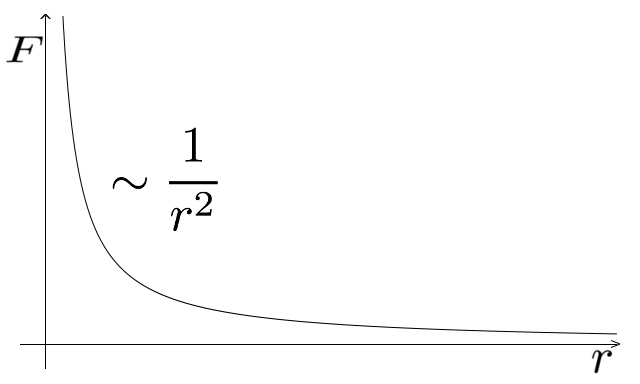
\includegraphics[scale=0.72]{forza_elettrica}
               \caption{\small{Grafico che relazione intesità di forza elettrica e distanza dalla fonte del campo.}}
               \end{figure} 
               \end{center}
               Si osserva come il grafico renda conto della diminuzione della forza con il crescere della distanza.
               \newpage
               Una carica puntiforme produce inoltre un campo di forze centrali:
               \begin{center}
\begin{figure}[H]
			  \vspace{-10pt}
              \hspace{-90pt}
              ~~~~~~~~~~~~~~~~~~~~~~~~~~~~~~~~~~ 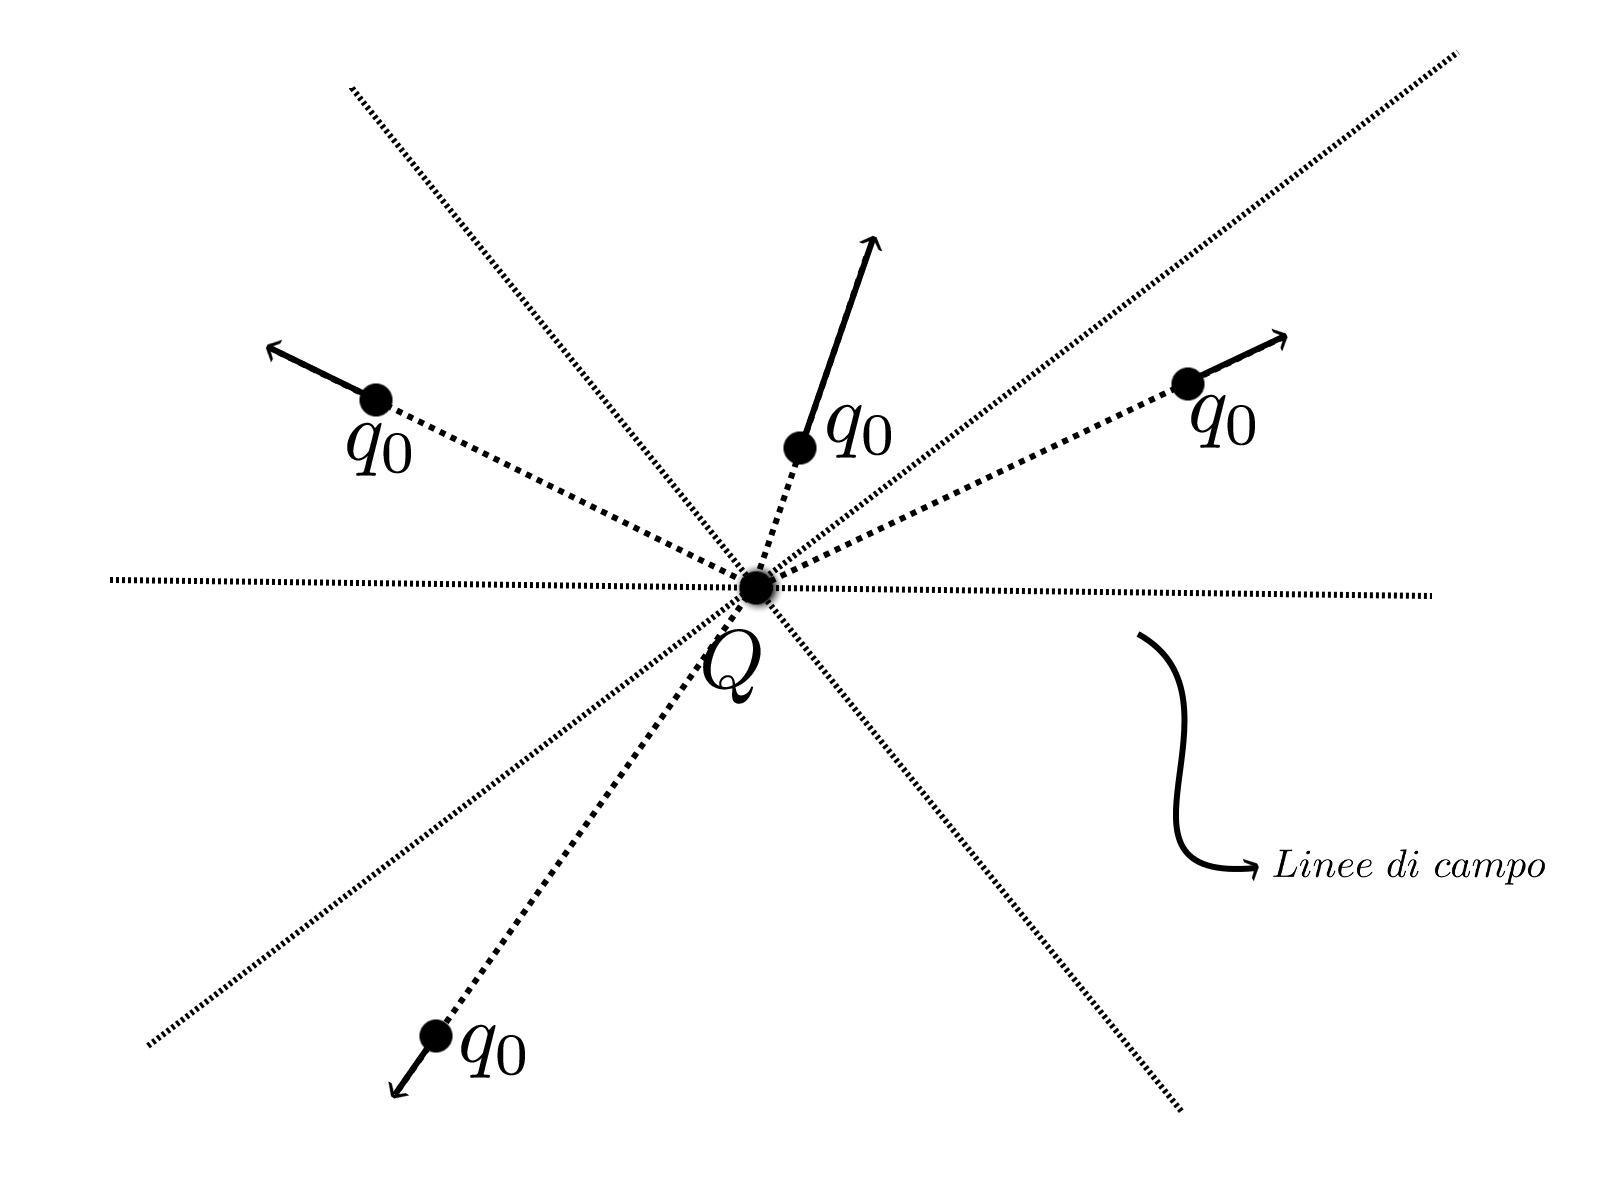
\includegraphics[scale=0.22]{campocentrale}
               \caption{\small{Rappresentazione del campo di forze generato da una carica puntiforme (con linee di campo).}}
               \end{figure} 
               \end{center}
Dal punto di vista teorico la carica di prova deve essere il più piccola possibile (poco carica) così da perturabare il sistema in modo trscurabile.
$$\overrightarrow{E}=\lim_{q_0\rightarrow 0}\frac{\overrightarrow{F}}{q_0}$$
\subsection{Distribuzione di cariche asimmetriche}
In generale un distribuzione di carica può essere particolare e assolutamente non si mmetrica. Consideremo campi elettrici generati da volumi, superfici, e linee aventi una determinata e nota densità di carica sotto l'unica ma fondamentale ipotesi di continuità di distribuzione della carica (vera fino ad un certo punto).
In generale per una distribuzione di carica qualsiasi, per il principio di sovrapposizione delle forze varrà:
\footnote{In questa trattazione la consueta notazione per i vettori ``$\overrightarrow{\nu}$'' sarà equivalente alla notazione ``$\overline{\nu}$''}$$\overline{E}=k_e\sum_{i=1}^{n}\frac{q_i}{|\overline{r}-\overline{r_i}|^2}\widehat{(\overline{r}-\overline{r_i})}=k_e\sum_{i=1}^{n}\frac{q_i(\overline{r}-\overline{r_i})}{|\overline{r}-\overline{r_i}|^3}$$
dove per $\widehat{(\overline{r}-\overline{r_i})}$ si intende il versore del vettore differenza tra $\overline{r}$ e $\overline{r_i}$.
\\\\Poichè in un caso generale (più reale) le cariche in gioco sono tantissime e molto vicine tra l'ora (almeno dal nostro punto di vista) occorre riformulare (reinventare) la formula appena scritta per renderla operativa.
Si introdurrà quindi la densità di carica, il differenziale volumico e quello di carica per poter ``passare al continuo'' sfruttando l'ipotesi verosimile della continuità della distribuzione della carica:
\newpage
Consideriamo una distribuzione generica di carica ed indichiamo con $d\tau$ il differenziale di volume di carica. Ipotizzando che la distribuzione di carica non sia omogenea ha senso considerare la funzione densitàa di carica $\rho(x,y,z)$ come la derivata $\frac{dq}{d\tau}$.
 \begin{center}
\begin{figure}[H]
			  \vspace{-10pt}
              \hspace{-90pt}
              ~~~~~~~~~~~~~~~~~~~~~~~~~~~~~~~~ 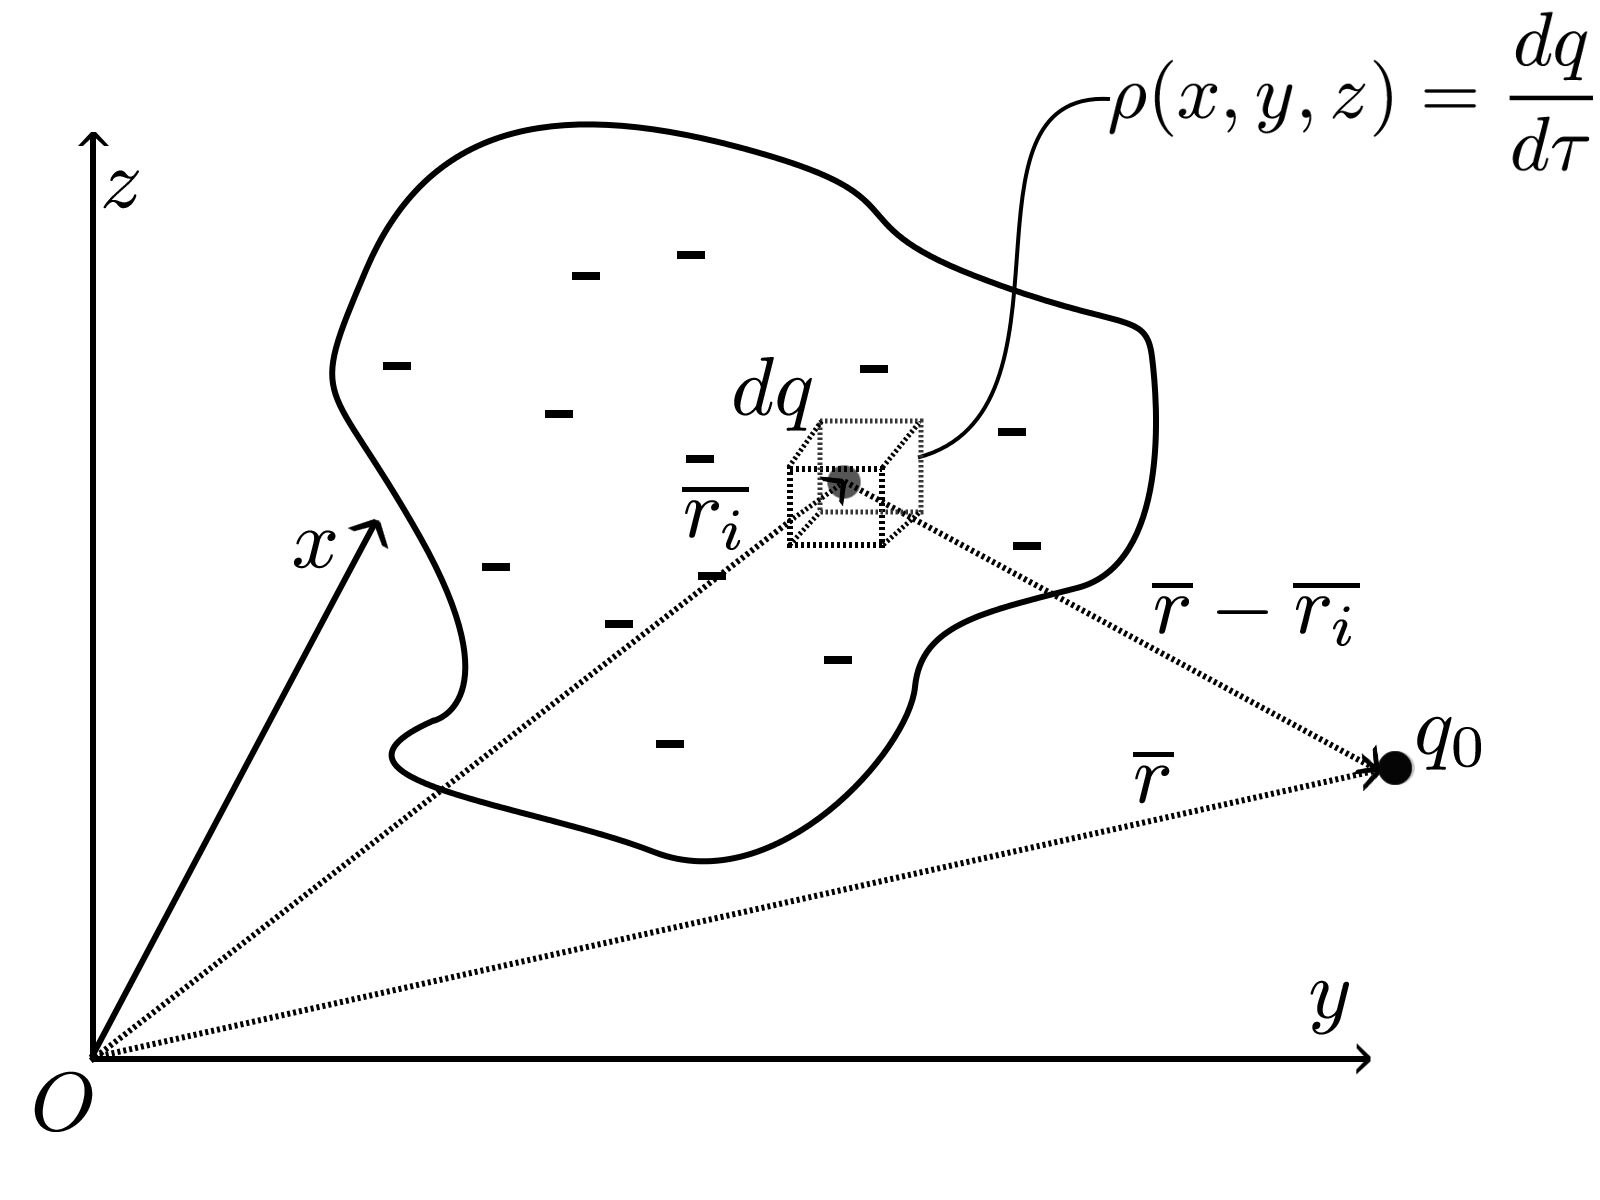
\includegraphics[scale=0.22]{distribuzione}
               \caption{\small{Distribuzione di carica generica.}}
               \end{figure} 
               \end{center}
               Con le notazioni in figura
PROVA MODIFICA push
\end{document}